\documentclass[12pt,a4paper]{article}
\usepackage[utf8]{inputenc}
\usepackage[czech]{babel}
\usepackage[T1]{fontenc}
\usepackage{amsmath}
\usepackage{amsfonts}
\usepackage{amssymb}
\usepackage{graphicx}
\usepackage{titlesec}
\usepackage[left=2cm,right=2cm,top=2cm,bottom=2cm]{geometry}
\usepackage{indentfirst}
\usepackage{listings}
\usepackage{color}

%Pravidlo pro řádkování
\renewcommand{\baselinestretch}{1.5}

%Pravidlo pro začínání kapitol na novém řádku
\let\oldsection\section
\renewcommand\section{\clearpage\oldsection}

%Formáty písem pro nadpisy (-změněno na bezpatkové \sffamily z původního \normalfont
\titleformat{\section}
{\sffamily\Large\bfseries}{\thesection}{1em}{}
\titleformat{\subsection}
{\sffamily\large\bfseries}{\thesubsection}{1em}{}
\titleformat{\subsubsection}
{\sffamily\normalsize\bfseries}{\thesubsubsection}{1em}{}

%Nastavení zvýrazňování kódu v \lslisting
\definecolor{mygreen}{rgb}{0,0.6,0}
\definecolor{mygray}{rgb}{0.5,0.5,0.5}
\lstset{commentstyle=\color{mygreen},keywordstyle=\color{blue},numberstyle=\tiny\color{mygray}}

\author{Jan Šmejkal}

\begin{document}

%-------------Úvodni strana---------------
\begin{titlepage}


\includegraphics[width=50mm]{img/FAV.jpg}
\\[160 pt]
\centerline{ \Huge \sc Semestrální práce z předmětu KIV/BIT}
\\[12 pt]
{\large \sc
\centerline{Implementace šifry SAFER K-64}
}


{
\vfill 
\parindent=0cm
\textbf{Jméno:} Jakub Záruba\\
\textbf{Osobní číslo:} A13B0476P\\
\textbf{E-mail:} eflyax@students.zcu.cz\\
\textbf{Datum:} {\large \today\par} %datum

}

\end{titlepage}

%------------------------------------------

%------------------Obsah-------------------
\newpage
\setcounter{page}{2}
\setcounter{tocdepth}{3}
\tableofcontents
%------------------------------------------

%--------------Text dokumentu--------------
{\section{O šifře SAFER}}
Šifra SAFER K-64 (Secure And FAST Encryption Routine, s 64bitovým klíčem), je bloková šifra s 64bitovým plaintextem. Šifra SAFER k-64 spadá do rodiny šifer SAFER, které navrhnul James Massey (jeden z návrhářů šifry IDEA). Poprvé byla publikována v roce 1993. Všechny algoritmy z rodiny SAFER jsou nepatentované a jsou k dispozici pro neomezené použití.

{\section{Popis algoritmů}}
Šifra používá \emph{r} identických šifrovacích kol (rounds). Tato šifra standardně používá 6 rounds, počet může být volitelný. Maximum je však 10. Pro zadaný 64 bitový klíč se vytvoří 2r + 1 podklíčů, které mají také 64 bitů. 2 klíče se vždy použijí v jednom šifrovacím kole (2r) a poslední klíč (+1) se použije pro výstupní transformaci.   
Uživatelem zvolený vstup a klíč je dlouhý 8 bajtů (64 bitů). 

{\subsection{Šifrování}}

\begin{itemize}  
\item \textbf{Vstup}: r, 6 $\leq$ r $\leq$ 10 ; 64 bitový text M = $m_{1}$ ... $m_{64}$ ; klíč K = $k_{1}$ ... $k_{64}$
\item \textbf{Výstup}: 64 bitový šifrovaný text (blok) Y = ($Y_{1}$, ..., $Y_{8}$) 
\end{itemize}

\begin{enumerate}
\item Výpočet podklíčů $K_{1}$, ... , $K_{8}$ , viz kapitola xyz
\item ($X_{1}$,$X_{2}$,...$X_{8}$) 
$\leftarrow$
($m_{1}$...$m_{8}$, $m_{9}$...$m_{16}$,...$m_{57}$...$m_{64}$).
\item Pro \emph{i} od 1 proveď akce: (XOR-addition, S-box, XOR-adittion, 3x lineární vrstvy)
\item

\begin{enumerate}
\item Pro \emph{j} = 1,4,5,8: $X_{j}$ $\leftarrow$ $X_{j}$ $\oplus$ $K_{2i-1}$|j|\\
Pro \emph{j} = 2,3,6,7: $X_{j}$ $\leftarrow$ $X_{j}$ $\boxplus$ $K_{2i-1}$|j|
\item Pro \emph{j} = 1,4,5,8: $X_{j}$ $\leftarrow$ S[$X_{j}$], Pro j = 2,3,6,7: $X_{j}$ $\leftarrow$ $S_{inv}$[$X_{j}$].

\item Pro \emph{j} = 1,4,5,8: $X_{j}$ $\leftarrow$ S[$X_{j}$] $\boxplus$ $K_{2i}$|j|. Pro j =2,3,6,7: $X_{j}$ $\leftarrow$ $X_{j}$ $\oplus$ $K_{2i}$|j|.

\item Pro \emph{j} = 1,3,5,7: ($X_{j}$, $X_{j+1}$) $\leftarrow$ \emph{f} ($X_{j}$, $X_{j+1}$)

\item ($Y_{1}$, $Y_{2}$) $\leftarrow$ \emph{f}($X_{1}$, $X_{3}$), ($Y_{3}$, $Y_{4}$) $\leftarrow$ \emph{f}($X_{5}$, $X_{7}$)

($Y_{5}$, $Y_{6}$) $\leftarrow$ \emph{f}($X_{2}$, $X_{4}$), ($Y_{7}$, $Y_{8}$) $\leftarrow$ \emph{f}($X_{6}$, $X_{8}$)
\\
Pro  \emph{j} od 1 do 8 proveď: $X_{j}$ $\leftarrow$ $Y_{j}$
\item ($Y_{1}$, $Y_{2}$) $\leftarrow$ \emph{f}($X_{1}$,$X_{3}$), ($Y_{3}$, $Y_{4}$) $\leftarrow$ \emph{f}($X_{5}$,$X_{7}$)

($Y_{5}$, $Y_{6}$) $\leftarrow$ \emph{f}($X_{2}$,$X_{4}$), ($Y_{7}$, $Y_{8}$) $\leftarrow$ \emph{f}($X_{6}$,$X_{8}$)\\
Pro \emph{j} od 1 do 8 proveď: $X_{i}$ $\leftarrow$ $Y_{j}$
\end{enumerate}

\item Výstupní transformace:\\
Pro \emph{j} = 1,4,5,8: $Y_{j}$ $\leftarrow$ $X_{j}$ $\oplus$ $K_{2r+1}$|j|.\\
Pro \emph{j} = 2,3,6,7: $Y_{j}$ $\leftarrow$ $X_{j}$ $\boxplus$ $K_{2r+1}$|j|
\end{enumerate}

\begin{figure}
    \center
    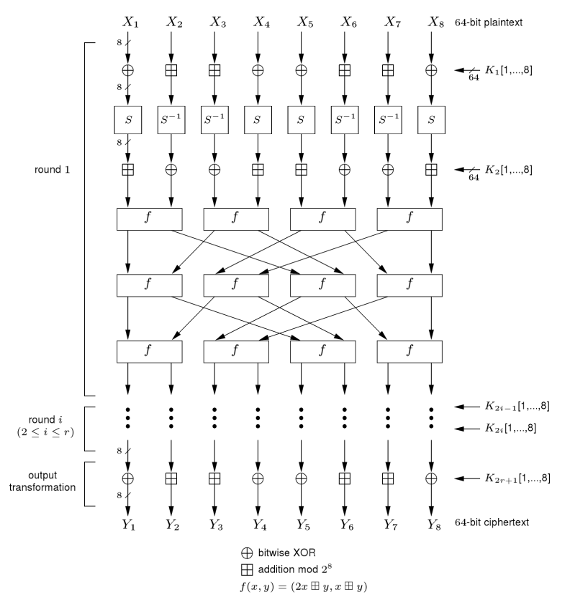
\includegraphics[width=120mm]{img/saferschema.png}
    \caption{Schéma šifrování}
\end{figure}


{\subsection{Produkce podklíčů}}
\begin{itemize}
\item \textbf{Vstup:} 64 bitový klíč K = $k_{1}$ ... $k_{64}$ ; počet šifrovacích kol \textbf{\emph{r}}
\item \textbf{Výstup:} 64 bitové podklíče $K_{1}$,...$K_{2r+1}$
\end{itemize}


\begin{enumerate}
\item Nechť R[\emph{i}] představuje 8 bitové úložiště dat a nechť $B_{i}$[\emph{j}] představuje bajt \emph{j} v $B_{i}$
\item (R[1], R[2], ... R[8]) $\leftarrow$ ($k_{1}...k_{8},k_{9}...k_{16},...,k_{57}...k_{64}$)
\item Pro \emph{i} od 2 do \emph{2r+1} proveď: 
\begin{enumerate}
\item Pro \emph{j} od 1 do 8 proveď: R[\emph{j}] $\leftarrow$ (R[\emph{j}] $\leftarrow$ 3)
\item Pro \emph{j} od 1 do 8 proveď: $K_{i}$[\emph{j}] $\leftarrow$ R[\emph{j}] $\boxplus$ $B_{i}$[\emph{j}]
\end{enumerate}
\end{enumerate}

\subsection{Dešifrování}
Proces dešifrování používá pro zadaný klíč K stejné hledání podklíčů, jako při šifrování. Proces začíná s se vstupní transformací s klíčem $K_{2r+1}$ k výstupní transformaci. Veškeré modulární součty jsou nahrazeny modulárním odečítáním.
Funkce \emph{f} v lineárních vrstvách jsou nahrazeny jejich inverzními funkcemi: $\emph{f}_{inv}$(L,R) = (L - R, 2R - L) s odečítáním mod 256 v tříkrokových sekvencích.



{\section{Popis implementace}}


{\section{Závěr}}
Lorem ipsum dolor sit amet, consectetuer adipiscing elit. Pellentesque habitant morbi tristique senectus et netus et malesuada fames ac turpis egestas.

%------------------------------------------

\end{document}